\documentclass{beamer}
\usetheme{default}
\begin{document}

\begin{frame}{Introduction}
\begin{center}
  An Image Classifier

  Brendan Miller
\end{center}

\begin{itemize}
  \item An image classifier based on the generative/discriminative framework
  presented in Yi Li's paper.
  \item A ``bag of words'' classifier.
  \item Uses SIFT key-point descriptors and color.
\end{itemize}

\end{frame}

\begin{frame}{Basic Idea}
  A quick high level summary of Li's classification framework:
  \begin{itemize}
    \item Build a mixture model of features in an images containing a class of objects.
    \item Determine how well a training set of images match each component of the model.
    \item Build a vector of these match values (joint probabilities).
    \item Use these values as the inputs to train a classifier (a neural network).
  \end{itemize}
\end{frame}

\begin{frame}{Generative/discriminative model part 1}

Generative model.

\begin{itemize}
  \item Gaussian mixture model of distribution of features constructed using EM algorithm.
    \begin{equation*}
      P(X^a|o) = \sum_{m=1}^{M^a} w^a_m N(X^a; \mu^a_m, \Sigma^a_m)
    \end{equation*}
  \item Joint probability of image features with each model component is calculated.
    \begin{equation*}
      P(X^a_{i,r},m^a) = w^a_m N(X^a_{i,r}, \mu^a_m, \Sigma^a_m)
    \end{equation*}
  \item For each image and gaussian component, the maximum joint probability is found.
    \begin{equation*}
      P(I_i, m^a) = max(\{P(X^a_{i,r}, m^a)|r \in \mbox{features of type $a$
        in the $i$th image\}})
    \end{equation*}

\end{itemize}  

\end{frame}

\begin{frame}{Generative/discriminative model part 2}

Discriminative classifier.

\begin{itemize}
  \item The maximum joint probabilities are used as inputs to train a neural network.
  \item The neural network acts as a classifier.
  \item The classifier understands not just how well an example image
    fit the (mixture of gaussians) model, but how well it fit
    \emph{each component} of the model.
  \item Some components of the model found during the generative phase
    may also be present in images which do not contain the object we
    are looking for. Some components may be necessary but not
    sufficient to establish the presence of an object. The
    discriminative phase deals with these problems.
\end{itemize}
\end{frame}

\begin{frame}{Features}
\begin{itemize}
  \item Original paper used regional features e.g. color, texture.
  \item My project also uses key-point descripters i.e. SIFT.
  \item I also keep color. Mainly useful for improving accuracy on
    face detection where color can detect the distinctive skin tone.
  \item Color is not that useful for classifying cars, planes,
    motorcycles which may be painted any color.
\end{itemize}    
\end{frame}

\begin{frame}{SIFT}
\begin{itemize}
  \item SIFT alone produces good results.
  \item Increasing the number of Gaussian components (50+) helps accuracy.
  \item Objects are made of many parts. Ideally each Gaussian
    component matches a part.
\end{itemize}    
\end{frame}

\begin{frame}{Correct classification}
  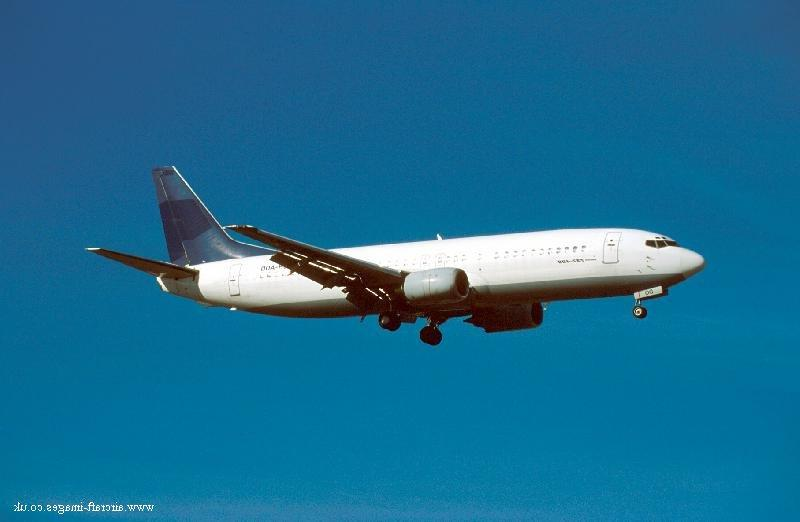
\includegraphics[width=100mm]{images/plane_true_positive.png}
\end{frame}

\begin{frame}{False Negative}
  Face detection more reliant on color than others.
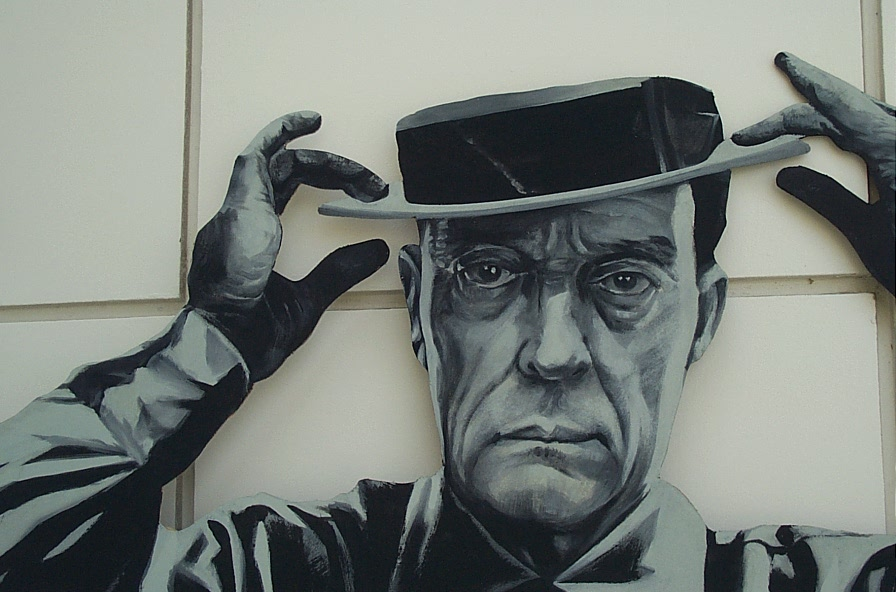
\includegraphics[width=100mm]{images/face_false_negative.png}
\end{frame}

\begin{frame}{Accuracy}
\begin{tabular}{| l | l | l | l |}
  \hline
  Image Type & Accuracy     & False Positives    & False Negatives \\
  Cars      & 0.94  & 0.035 & 0.025 \\
  Planes    & 0.78  & 0.11  & 0.11  \\
  Faces     & 0.9   & 0.055 & 0.045 \\
  Bikes     & 0.805 & 0.08  & 0.115 \\
  \hline
\end{tabular}
\end{frame}

\begin{frame}{Future work}
\begin{itemize}
  \item One idea: How can we find which parts of an image contain the classified object?
  \item Given a classified image, it would be nice to be able to work
    backwards and find the features which contributed the most to the
    classification.
  \item Given the most important features, a bounding box could be created.
  \item A 3 layer neural network might not be ideal for this. It would
    be easier to work backwards through a simpler classifier.
\end{itemize}

\end{frame}

\end{document}